\documentclass[12pt]{article}

\usepackage{geometry} 
\usepackage{authblk}
\usepackage{hyperref}
\usepackage[parfill]{parskip}

\usepackage{graphicx}
\graphicspath{ {./} }

\geometry{a4paper}   


\usepackage{titling}
\setlength{\droptitle}{-4em}


\title{Ongoing Blockchain Research}
\author{Misrab M. Faizullah Khan}

\affil[]{Orion Labs}

\affil[]{\href{mailto:faizullah.misrab@gmail.com}{faizullah.misrab@gmail.com}}


\date{December 2017}
%Koç University Computer Engineering Department


\begin{document}
\maketitle


\section*{Title}

Which came first, the storage or the compute? An alternative paradigm to Ethereum for scalable blockchain applications, using IPFS and Filecoin.

\section*{Introduction and Literature}

Traditional Proof-of-Work blockchains \cite{bitcoin}, such as Ethereum \cite{ethereum} in its current state, require each node in the network to process each transaction. If $c$ denotes the computational capacity of a single node, transaction capacity is then bounded by $O(c)$. This currently translates to about 10 transactions per second \cite{ethereum-tps}, with modest applications running into bottlenecks \cite{cryptokitties}.

For most applications to become mainstream, several orders of magnitude improvement will be required. There are a few approaches to solving this problem, including: payment channels \cite{lightning}, more general state channels \cite{plasma}, and sharding. This last approach is often seen as the holy grail of scalability, and takes several forms such as purely transactional sharding \cite{elastico}, quadratic transaction and storage sharding, and the more challenging super-quadratic sharding \cite{sharding}.

All of the above methods conform to the prevalent blockchain paradigm: build a protocol that manages fundamentals like peer-to-peer networking, transaction processing, and state; start with the simplest form of Nakamoto consensus \cite{nakamoto}; evolve the protocol to gradually introduce scalability.

There is however an alternative paradigm: smart contracts built on top of IPFS \cite{ipfs} and Filecoin \cite{filecoin}. In this universe, the building blocks of peer-to-peer networking and content-addressed storage over a DHT \cite{dht} are first solved. Next, consensus based on useful work through Proof-of-Storage (name Proof-of-Replication and Spacetime \cite{porep}) enables an incentivised distributed storage system. Most interestingly, one can then construct a wide range of sharded consensus systems using only \textit{Put} and \textit{Get} primitives, without reinventing the building blocks. Smart contract code can be deployed with arbitrary redundancy, and contract state can be stored on the same or different nodes. This is illustrated in one of many possible ways below. It is worth noting that the consensus mechanism is not specified here: IPFS allows for a blockchain, or more general Merkle \cite{merkle} tree structures.

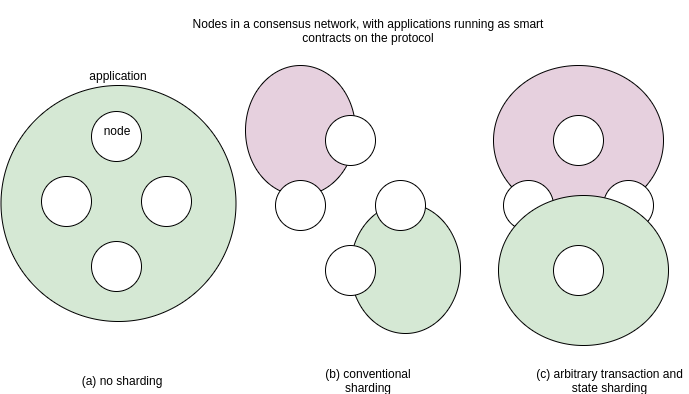
\includegraphics[width=\textwidth]{sharding}

The aim of this research will be to explore the spectrum of consensus architectures for smart contract applications on top of such a system, alongside their performance (scalability, safety, liveness) and security (incentive-compatibility) characteristics. In the simplest extreme, one could replicate Nakamoto consensus on top of IPFS and Filecoin. On the other hand, one could tune the degrees of sharding based on application-specific requirements. This provides an exciting alternative to the current one-size-fits-all approach, and is an avenue certainly worth exploring.


\section*{Results and Impact}

At the end of this research, we should have a classical distributed system understanding of the characteristics of several consensus approaches on top of IPFS and Filecoin, a game-theoretic view of security through incentive compatibility, as well as the consequences on high-level application design.

It is no understatement that distributed ledger technology can fundamentally revolutionise power structures and markets. Yet the field is still highly experimental, and it remains to be seen what dominant consensus mechanisms emerge. Now is a perfect time to explore different paradigms with an open mind, and develop a sound theoretical and practical understanding of the tradeoffs involved.



\medskip
 
\begin{thebibliography}{13}

\bibitem{bitcoin}
Bitcoin Proof-of-Work, 
\href{https://bitcoin.org/bitcoin.pdf}{https://bitcoin.org/bitcoin.pdf}

\bibitem{ethereum}
Ethereum White Paper, 
\href{https://github.com/ethereum/wiki/wiki/White-Paper}{https://github.com/ethereum/wiki/wiki/White-Paper}

\bibitem{ethereum-tps}
Ethereum Transaction Bottleneck, 
\href{https://twitter.com/VitalikButerin/status/940749096339542016}{https://twitter.com/VitalikButerin/status/940749096339542016}

\bibitem{cryptokitties}
Cryptokitties Congestion, 
\href{https://qz.com/1145833/cryptokitties-is-causing-ethereum-network-congestion/}{https://qz.com/1145833/cryptokitties-is-causing-ethereum-network-congestion/}

\bibitem{lightning}
Lightning Network, 
\href{https://lightning.network/}{https://lightning.network/}

\bibitem{plasma}
Plasma, 
\href{https://plasma.io/}{https://plasma.io/}

\bibitem{elastico}
Elastico, 
\href{https://www.comp.nus.edu.sg/~loiluu/papers/elastico.pdf}{https://www.comp.nus.edu.sg/~loiluu/papers/elastico.pdf}

\bibitem{sharding}
Ethereum Sharding, 
\href{https://github.com/ethereum/sharding/blob/develop/docs/doc.md}{https://github.com/ethereum/sharding/blob/develop/docs/doc.md}

\bibitem{nakamoto}
Nakamoto Consensus, 
\href{https://www.quora.com/What-is-the-Nakamoto-consensus}{https://www.quora.com/What-is-the-Nakamoto-consensus}

\bibitem{ipfs}
The InterPlanetary File System, 
\href{https://ipfs.io/ipfs/QmR7GSQM93Cx5eAg6a6yRzNde1FQv7uL6X1o4k7zrJa3LX/ipfs.draft3.pdf}{https://ipfs.io/ipfs/QmR7GSQM93Cx5eAg6a6yRzNde1FQv7uL6X1o4k7zrJa3LX/ipfs.draft3.pdf}

\bibitem{filecoin}
Filecoin, 
\href{https://filecoin.io/filecoin.pdf}{https://filecoin.io/filecoin.pdf}

\bibitem{dht}
Distributed Hash Table (DHT), 
\href{https://github.com/ipfs/go-ipfs/issues/1396}{https://github.com/ipfs/go-ipfs/issues/1396}

\bibitem{porep}
Proof-of-Replication and Spacetime, 
\href{https://filecoin.io/proof-of-replication.pdf}{https://filecoin.io/proof-of-replication.pdf} 

\bibitem{merkle}
Merkle DAGs,
\href{https://github.com/ipfs/specs/tree/master/merkledag}{https://github.com/ipfs/specs/tree/master/merkledag}

\end{thebibliography}



\end{document}